\chapter{Team 3 Agent Design}\label{team_3_agent_design}

\section{Agent Implementation}
    
    \subsection{The Ideology}
        One can see the agent design ideology presented in this document as a computational implementation of the \textit{preference utilitarianism}. In this doctrine, it is assumed that the agent's decision-making is influenced by maximising personal interests, albeit complemented by a rational perspective on the progress of the game. Hence, the agent is capable of maximising personal satisfaction but also satisfies the rudimentary actions indispensable for the game to progress in the long run.\cite{jeremy}
        
        Needless to say, in the absence of trusted social counterparts, the agent must recognise an existential risk when extrapolating behavioural consequences of self-centred actions. Therefore, the environmental adaptability of the entity is also affected by social capital. In this context, it is to be understood as a constantly appending network of agent-to-agent interconnections, a process of forming natural bonds and \textit{storing} data about agents deemed to be trusted\footnote{later referred to as \textit{Trusted Social Network (TSN)}}.

        \begin{figure}[H]
            \centering
            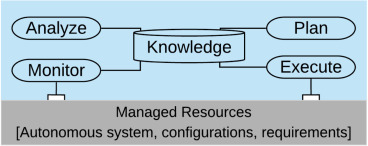
\includegraphics{006_team_3_agent_design/FIGS/mapek.jpg}
            \caption{MAPE-K framework}
            \label{fig:mapek_framework}
        \end{figure}

        The ideological architecture presented above falls within the assumption of the self-organising MAPE-K interaction framework\cite{mapek}. See figure \ref{fig:mapek_framework}. The agent monitors the environment to make the most balanced decision, with a strong personal incline as a general preference. On the other hand, it can detect anomalies, which can be perceived as a non-favourable outcome of a number of fight attempts. After all, the architecture concerned aims to plan a sequence of actions, to execute it to find itself in a 'better state'\footnote{which in this context might be related to improving internal parameters, or contributing to the commonwealth.} and to store knowledge between several autonomous elements. The latter one, as it will be shown later, shall fit into \textit{Ostrom's} perspective on the benefits of non-centralised governance, which in the context of multi-agent systems, may only function in the presence of ubiquitous common knowledge representation framework.

        In all, the agent shall contribute to society by taking an active part in conquering subsequent levels, at the same time being preferential towards its own benefits and its trusted social network.
        
        
    \subsection{Autonomous Decision-making}
        The agent's decision is based on a \textit{Semi-Reinforcement Social-Construct} learning algorithm. This approach benefits from the combination of a proven-to-be-effective weight-updating model with added efficiency from social interaction; all within the boundaries of freedom determined by the concept of open society, where every agent can, and indeed should manifest a proposal. In other words, these actions will be reinforced by social capital and collective risk analysis which, in fact, unites all agents to achieve the common goal: leaving the Pit(t).
        
        At this point, it is crucial to stress the function of social capital when it comes to \textit{reward} and \textit{punishment}. It is a form of recognition based on whether the fellow agent had a beneficial or detrimental effect on the individual. Furthermore, the collective risk analysis is based on an internal function of what is regarded as \textit{fairness} and \textit{effectiveness}. These metrics will be susceptible to a number of parameters extracted by getting into interaction with a particular entity, building rapport or simply evaluating the performance of a chair.
        
        Our agent will be evaluating the game and choose his action based on his knowledge and intuition of who is helping him, as well as one's general contribution to the collective. In the extreme case of an unfavourable position, it will be biased towards maximising self-satisfaction. The trade-off between short-run hedonism and long-term joint achievements will ultimately depend on, both, the current state, and the historical data which forms the agent's experience, knowledge and expectations regarding what is yet to come. 

\section{Social Interaction \& Utility Interpretation}

        One of the greatest challenges when working on the agent design was an algorithmic representation of the social capital, so that each bond between two entities, as well as social relations, not only can be represented as knowledge in the system but also capable of coming up with the most suitable action. It was decided to implement the utility function to make the computational representation as close as possible to the theoretical reasoning. It is used and updated by our agents to represent dynamically changing relations. Therefore, the utility score obtained is a list mapping the id of every agent to their utility\footnote{This ranges from 0 to 15}. The \textit{utility} is based on the aggregated weighted average of 3 actions:
        
        The first utility factor is related to \textit{trade interaction}. The agent introspectively punishes when the resource trade process is rejected and rewards when the resource is traded.
        The punishment parameter executing the \textit{retributive justice} (that is, the decrease in an internal \textit{trade utility} score) is different depending on the relationship with a particular 'transgressor' and the already established value of the utility parameter. This ensures that the punishment never breaks the bond with a fellow agent unless it is absolutely necessary due to its detrimental effect. For the same reason, the amount of reward is always higher than the punishment. This simple, yet effective \textit{forgiveness} implementation ensures extensive social capital and increases the chance to maintain the bond.
        
        The second factor relates to the performance of the proposal. If our agent had been asked about the fight decision that turned out to be identical to the individual asking, the \textit{proposal utility} parameter would increase. Otherwise, the score would decrease indicating a particular agent's worldview is askew. 
        
        The last function allows for a biased chair assessment. Hence, if the internal fight decision of our agent is different than what the proposal of the governor was,\footnote{and if he has the power for at least 4 rounds} its \textit{chair utility }score will decrease. Otherwise, it will always increase to bear in mind that this agent proved to have a suitable leading strategy through the perspective of our algorithm.
        
        To obtain an aggregate utility, both, chair and resource utilities are weighted equally. Due to the nature of round/level operation within the game, \textit{proposal utility} has a lower level of contribution to the weighted average. The main reason behind that decision is the \textit{participation principle}, and the implication that the decision frequency is lower than its application. On the final note, as shown below, agents' utility scores are capped at 15 and cannot go below 0.



\begin{algorithm}
\caption{Resource utility}
\begin{algorithmic} 
\Require $agent\_id, resource\_utility$
\Ensure $resource\_utility\_output[0-15]$
\If{Initial State}
\State $resource\_utility \leftarrow 7$
\EndIf
\If{Trade Rejected}
\If{$resource\_utility \geq 12$}
\State $resource\_utility \leftarrow resource\_utility-1$
\EndIf
\If{$ 7 \leq resource\_utility < 12$}
\State $resource\_utility \leftarrow resource\_utility-2$
\Else
\State $resource\_utility \leftarrow resource\_utility-3$
\EndIf
\EndIf
\If{Trade Accepted}
\State $resource\_utility \leftarrow resource\_utility+3$
\EndIf
\end{algorithmic}
\end{algorithm}


\begin{algorithm}
\caption{Proposal utility}
\begin{algorithmic} 
\Require $agent\_id, proposal\_utility$
\Ensure $proposal\_utility\_output[0-15]$
\If{Initial State}
\State $proposal\_utility \leftarrow 7$
\State $ACC \leftarrow 0$
\EndIf
\If{Asked About Proposal $\land$ This Proposal Holds $\land ~\neg$Our Decision}
\State $ACC \leftarrow ACC+1$
\If{$ACC = 3$}
\State $proposal\_utility \leftarrow proposal\_utility - 1$
\State $ACC \leftarrow 0$
\EndIf
\EndIf
\If{Asked About Proposal $\land$ This Proposal Holds $\land$ Our Decision}
\State $proposal\_utility \leftarrow proposal\_utility + 1$
\EndIf
\end{algorithmic}
\end{algorithm}

%acc go to 0 everytime it changes chair
\begin{algorithm}
\caption{Chair utility}
\begin{algorithmic} 
\Require $agent\_id, chair\_utility$
\Ensure $chair\_utility\_output[0-15]$
\If{Initial State}
\State $chair\_utility \leftarrow 7$
\State $ACC \leftarrow 0$
\EndIf
\If{Asked About Fight Decision}
\If{Agent Decision $\neq$ Our Decision}
\State $ACC \leftarrow ACC+1$
\If{$ACC = 4$}
\State $chair\_utility \leftarrow chair\_utility - 1$
\State $ACC \leftarrow 0$
\EndIf
\EndIf
\If{Agent Decision $=$ Our Decision}
\State $chair\_utility \leftarrow chair\_utility + 1$
\EndIf
\EndIf
\end{algorithmic}
\end{algorithm}

\begin{algorithm}
\caption{Total Utility}
\begin{algorithmic} 
\Require $agent\_id, chair\_utility, resource\_utility, proposal\_utility$
\Ensure $total\_utility\_output[0-15]$
\If{End of Round}
\State $total\_utility \leftarrow average\{chair\_utility \times 0.45, resource\_utility \times 0.45, proposal\_utility \times 0.10\}$
\EndIf
\end{algorithmic}
\end{algorithm}


\clearpage
\section{Borda Count for Distributive Justice }

Canons of judicial conduct, $C_0$ : \textit{Needs} and $C_1$ : \textit{Productivity}, with their effects on the commonwealth, are measured and reinforced through the process of updating respective weights. These are the most viable features for our design, both given a constant value of 5 as an initial condition for every fellow agent. As per the algorithm presented below, weights for these will be updated accordingly, thereby forming a plausible metric indispensable for suitable decision-making.

The final \textit{borda score} returned for each agent can be further used as a viable representation of \textit{fairness}. Hence, the agent framework could be sorted based on the fairness level, thereby implementing the principle of \textit{Borda Voter}.

It suffices to note that $w_1$ is updated according to the health and stamina of each agent, whereas $w_2$ is changed by a simple fact, whether an agent was active in battle\footnote{fought or defended actively} or just cowered.

\begin{algorithm}
\caption{Borda Score}
\begin{algorithmic} 
\Require $agentMap, w_1, w_2, needs, productivity$
\While{}{$i$ in $agentMap$}
\State $Update Weights$
\State $Score \leftarrow w_1 \times needs + w_2 \times productivity$
\State $fairness[agentID] \leftarrow Score$
\EndWhile
\State $sort(fairness)$\\
\Return FAIRNESS
\end{algorithmic}
\end{algorithm}


\begin{algorithm}
\caption{Update Weights [W1]}
\begin{algorithmic} 
\Require $agentMap, healthINIT, staminaINIT,healthNOW, staminaNOW$
\State healthINIT $\leftarrow agentMap.healthINIT.ALL$
\State staminaINIT $\leftarrow agentMap.staminaINIT.ALL$
\If{$updateW1$}
\State healthNOW $\leftarrow$ health from thread
\State staminaNOW $\leftarrow$ stamina from thread
\State HP $\leftarrow$ healthINIT[agent.ID] $-$ healthNOW[agent.ID]
\State ST $\leftarrow$ staminaINIT[agent.ID] $-$ staminaNOW[agent.ID]
\If{$ST>0$}
\State $W1~+= 0.2$
\Else
\State $W1~-= 0.2$
\EndIf
\If{$HP>0$}
\State $W1~+= 0.2$
\Else
\If{$HP = 0$}
\State $W1 = W1$
\Else
\State $W1 -= 0.2$
\EndIf
\State $W1~-= 0.2$
\EndIf
\If{$W1>10$}
\State $W1=10$
\EndIf
\If{$W1<0$}
\State $W1 = 0$
\EndIf
\State healthINIT[agent.ID] $=$ healthNOW
\State staminaINIT[agent.ID] $=$ staminaNOW
\Return W1
\EndIf
\end{algorithmic}
\end{algorithm}


\begin{algorithm}
\caption{Update Weights [W2]}
\begin{algorithmic} 
\Require $agentMap, healthINIT, staminaINIT,healthNOW, staminaNOW$
\If{agentFoughtAndDefended}
\State $W2~+= 0.2$
\Else
\State $W2~-= 0.2$
\EndIf
\If{$W2<0$}
\State $W2 = 0$
\EndIf
\If{$W2>10$}
\State $W2 = 10$
\EndIf
\State
\Return W2
\end{algorithmic}
\end{algorithm}


\clearpage
\section{Agent Operation Cycle}

All agent functionalities shown in the form of the game cycle graph are presented in figure \ref{fig:agent_model}. After each level commences the agent makes a decision regarding a donation to the common pool resources. Later, a sequence of decisions must be taken starting from the fight or flight, finishing on the resource trade and governance approach.

\begin{figure}[H]
    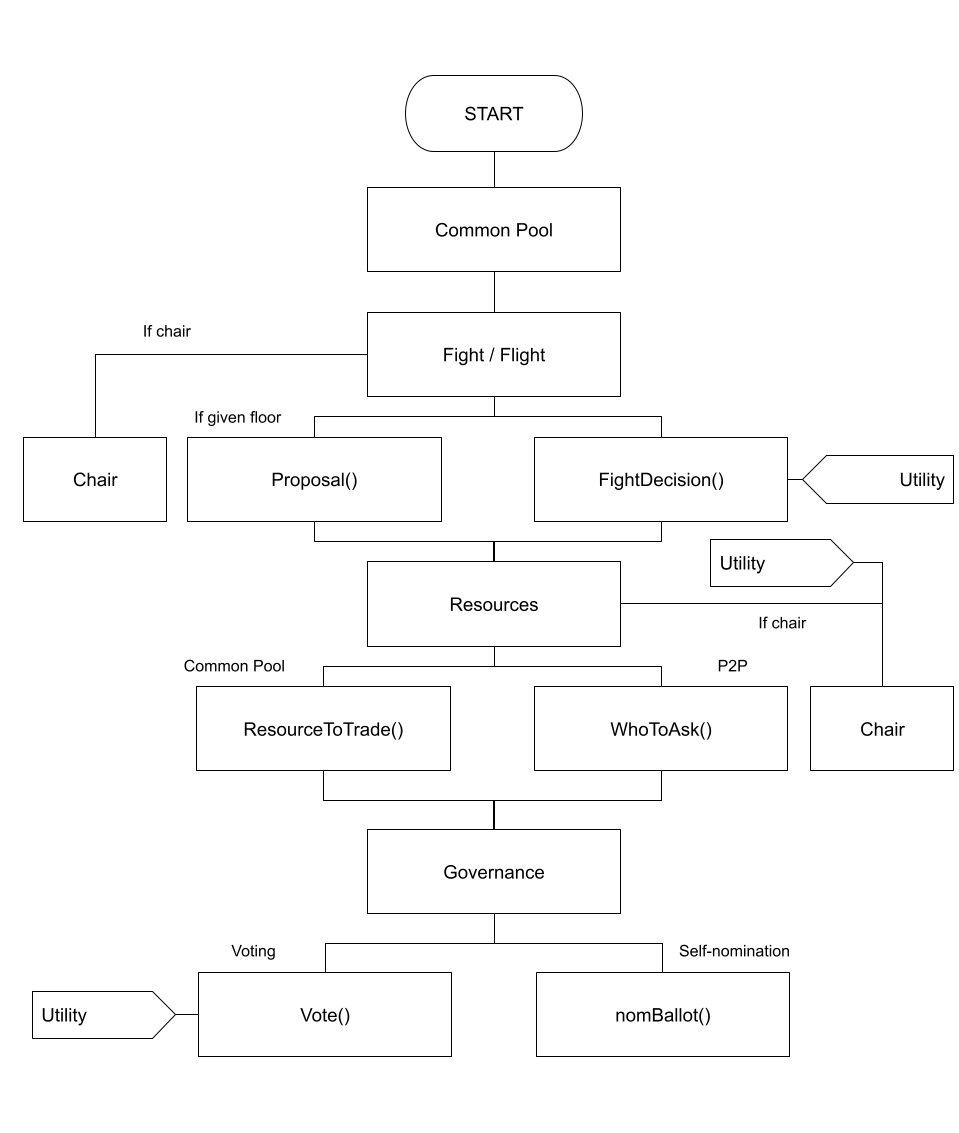
\includegraphics[scale=0.35]{006_team_3_agent_design/FIGS/diagram.png}
    \caption{Agent Model Draft}
    \label{fig:agent_model}
\end{figure}

\clearpage


\section{Fight, Defend \& Cower Decision}


%MODIfIED:

Arguably, the decision about agent allocation as a fight resource is the most essential in the game. It can be perceived as an individual preference, as well as joint distribution based on social will. In this section the internal fight decision-making process will be discussed, followed by the proposal formation technique.


\subsection{Internal fight decision}
    The first part is an internal function to see if our agent is going to fight or flee. In this part, the Health points, resource confidence\footnote{attack, shield} and the number of cowering decisions until the current state.
    To maximise self-satisfaction and avoid jeopardy, the agent will always cower if its health point is smaller  than  1.25 $\times$ average(HP) of the agents or 1.25 $\times$ stamina(HP). Otherwise, based on which resource confidence is higher, it will defend or attack as outlined below.

    On the other hand, if our agent is not in the internally-defined edge case\footnote{that is, it has not a critically low level of parameters required to survive the round}, and he has cowered for more than $\alpha$\footnote{starting with $\alpha~=~3$} rounds, it will fight. The accumulator parameter $\alpha$ will be increased continuously every 3 levels by 1; hence, the agent becomes more selfish the more levels increase.


    \begin{algorithm}
    \caption{Internal Fight Decision}
    \begin{algorithmic} 
    \Require $agent\_id, HP\_total, HP, Damage, Shield$
    \Ensure Possible to vote
    \If{$HP < 1.05 \times average(HP\_total) \lor Stamina < 1.05 \times average(STAMINA\_total)$}
    \Return COWER
    \EndIf
     \If{$Shield \leq Damage$}
    \Return ATTACK
    \EndIf
    \If{$Shield > Damage$}
    \Return DEFEND
    \EndIf
    \end{algorithmic}
    \end{algorithm}
    
    
    \begin{algorithm}
    \caption{Edge Case}
    \begin{algorithmic} 
    \Require $agent\_id, HP\_total,Stamina\_total, HP, Stamina, Damage, Shield$
    %\Ensure $Possible\_to\_vote$
    
    \If{$Stamina < 0.6*average(Stamina\_total) \lor HP < 0.6*average(HP\_total)$}
    \Return COWER
    \EndIf
    \end{algorithmic}
    \end{algorithm}
    
    \begin{algorithm}
    \caption{Change Decision}
    \begin{algorithmic} 
    \Require $agent\_id, HP\_total, HP, Damage, Shield$
    \Ensure $Possible\_to\_vote$, $\alpha$ initially 0, increments every 5 rounds
    \If{$\neg EdgeCase()$}
    \If{$AD \leq DT \land round \geq \alpha+3$}
    \Return ATTACK
    \If{$AD > DT \land round \geq \alpha+3$}
    \Return DEFEND
    \EndIf
    \EndIf
    \EndIf
    \end{algorithmic}
    \end{algorithm}
    \pagebreak

\subsection{Threshold Proposal for Fight Decision}
    
    The second fight decision is required to form a viable proposal based on the internal needs and necessary actions for the collective to succeed. In all, in this design agent must operate on 6 thresholds; three for the \textit{Attack}\footnote{this concerns HP, Stamina, BonusAttack} and three for the \textit{Defence}\footnote{this concerns Stamina and BonusDefence only}. These will be used to effectively obtain the proposal map which defines each agent's desired state for the level. There are three factors that impact the value of the proposal thresholds.
    
    \begin{itemize}
    \item The first one is based on the internal agent's decision. 
    It was decided that if our agent cowers, but is currently in a good state\footnote{which would still allow it to fight}, then the HP and Stamina threshold for people to attack or defend should be lower than the social average. However, if our agent wants to cower and he is in bad shape, the HP and Stamina threshold for the proposal could, in fact, be higher than the average. For the attack and defend threshold, we will propose approximately the average value be in place.
    On the other hand, if an agent decides to fight, then he will ask for an average threshold, as it is beneficial for a higher proportion of agents to fight in order to distribute the damage.

    \item The second threshold is based on the agent's trusted social network decision to fight or flight. If more than half of the group of agents we have established a bond with want to fight, the threshold is less than the average. Otherwise, it remains as before. If there is no reply from anyone in the TSN, then threshold 1 will hold. Otherwise, the weighted average of \textit{Threshold2} will be chosen, bearing in mind a substantially higher weight for the first one; that is, our agent's internal decision.
    
    \item Ultimately, the third threshold is a metric taking into consideration a group of agents from 3 different categories. These are to be understood as a social classification of individuals who, either, have the highest needs, are 'neutral' in the context of social capital, or are simply non-effective free-riders. 
    Based on the sorted array of agents, thanks to the Borda score, it is possible to establish the threshold. Even though this might be seen as a relatively convoluted way of gathering data about social behaviour, it allows for establishing a just collective action without an undesirable elitism component.
    \end{itemize}

\clearpage






\clearpage

\begin{algorithm}
\caption{Threshold Decision (Part 1)}
\begin{algorithmic} 
\Require $agent\_id, HP\_total, HP, Damage, Shield$
%\Ensure $Possible\_to\_vote$
\If{$ourHP \geq average(HP\_total) \land decision = COWER$}
\State $HPthreshold1 \leftarrow 1.7 \times average(HP\_total)$
\EndIf
\If{$ourSTAMINA \geq average(STAMINA\_total) \land decision = COWER$}
\State $STAMINAthreshold1 \leftarrow 1.7 \times average(STAMINA\_total)$
\EndIf
\If{$ourHP < average(HP\_total) \land decision = COWER$}
\State $HPthreshold1 \leftarrow 0.7 \times average(HP\_total)$
\EndIf
\If{$ourSTAMINA < average(STAMINA\_total) \land decision = COWER$}
\State $STAMINAthreshold1 \leftarrow 0.7 \times average(STAMINA\_total)$
\EndIf
\end{algorithmic}
\end{algorithm}

\begin{algorithm}
\caption{Threshold Decision (Part 2)}
\begin{algorithmic} 
\Require $agent\_id, HP\_total, HP, Damage, Shield$
%\Ensure $Possible\_to\_vote$
\If{Decision $=$ COWER}
\State $AttackThreshold1 \leftarrow 1.1 \times average(attackPoint)$
\State $Defence \leftarrow 1.1 \times average(defencePoint)$
\EndIf
% \Else
\If{Agent Fights}
\State $HPthreshold1 \leftarrow average(HP\_toral)$
\State $STAMINAThreshold1 \leftarrow average(STAMINA\_total)$
\State $AttackThreshold1 \leftarrow 0.4 \times average(ATTACK\_total)$
\State $DefenceThreshold1 \leftarrow 0.4 \times average(DEFENCE\_total)$
\EndIf
\If{$\geq50\%$~TSN want to fight}
\State $HPthreshold2 \leftarrow 0.7 \times average(HP\_toral)$
\State $STAMINAThreshold2 \leftarrow 0.7 \times average(STAMINA\_total)$
\State $AttackThreshold2 \leftarrow 0.6 \times average(ATTACK\_total)$
\State $DefenceThreshold2 \leftarrow 0.6 \times average(DEFENCE\_total)$
\EndIf
\If{$<50\%$~TSN want to fight}
\State $HPthreshold2 \leftarrow 1.1 \times average(HP\_toral)$
\State $STAMINAThreshold2 \leftarrow 1.1 \times average(STAMINA\_total)$
\State $AttackThreshold2 \leftarrow 1.1 \times average(ATTACK\_total)$
\State $DefenceThreshold2 \leftarrow 1.1 \times average(DEFENCE\_total)$
\EndIf
\If{NO REPLY FROM TSN}
\State Only use $threshold1$
\EndIf
\If{REPLY FROM TSN}
\State $0.8\times threshold1 + 0.2 \times threshold2$
\EndIf
\If{The agent asked $\geq$ 10\% of fellow agents}
\State $1.1 \times (0.8\times threshold1 + 0.2 \times threshold2)$
\EndIf
\If{The agent asked $<$ 10\% of fellow agents}
\State $0.9 \times (0.8\times threshold1 + 0.2 \times threshold2)$
\EndIf
\end{algorithmic}
\end{algorithm}

\vspace{1cm}
  

\vspace{1cm}



\begin{algorithm}
\caption{Proposal Agreement}
\begin{algorithmic}
\Require $agent\_id, HP\_total, HP, Damage, Shield$
\If{Proposal Agreement}
\If{$thresholdHP < 1.1 \times thresholdHPProposal \land thresholdHP > 0.9 \times thresholdHPProposal$}
\If{$thresholdStamina < 1.1 \times thresholdStaminaProposal \land
thresholdStamina > 0.9 \times thresholdStaminaProposal$}
\If{$thresholdAttack < 1.1 \times thresholdAttackProposal \land thresholdAttack > 0.9 \times thresholdAttackProposal$}
\If{$thresholdDefend < 1.1 \times thresholdDefendProposal \land thresholdDefend > 0.9 \times thresholdDefendProposal$}\\
\Return ACCEPT
\Else\\
\Return REJECT
\EndIf
\EndIf
\EndIf
\EndIf
\EndIf
\end{algorithmic}
\end{algorithm}

\clearpage
\section{Voting Decision}

The concept of institutionalised power and the need for self-organisation has been briefly signposted in the very first section of this agent-design document. Elinor Ostrom's set of working rules directed towards an institution for all self-governing agent commons was a principal bearing for the established voting approach. In the \textit{linear-public-goods-type} game, where the resources are scarce and profiles, just like in this design approach, preferentially individualistic, it is essential to form voting decisions whose focal point is narrowed onto several parameters; the effectiveness measure, the Trusted-Network-benefit, and the Agent-benefit. That is because, in an ideal case, each individual should be 'satisficed' with a good-enough solution to, both, survive and enhance the commonwealth. That, in the long-run should drastically increase the chances a positive outcome of the game.

The first one measures the effectiveness of the chair by directly measuring the increase in casualties in each subsequent level\footnote{this corresponds to a particular agent's 'reign' time}. Hence, if more agents died on the given level $N$ than $(N-i)$, where $i \in$ \{levels on which the chair was governing\}, then the chair of this level was less effective than the chair of the concerned beforehand.

The trusted-network-benefit parameter is true if and only if the current chair is part of the agent's TSN. This is to verify whetherer the potentially unfavourable decision of the governor should be condoned due to the already established relationship. Secondly, the agent-benefit parameter aims to measure if the current chair's actions aligh with the following:

\begin{enumerate}
    \item If for our agent $X$ and its internal decision $Y$ the resultant joint vote outcome is $Z$ then the following holds
    \begin{equation}
        \exists x, \forall y, \forall z, (y(x) \rightarrow z) \rightarrow agent\_benefit = true
    \end{equation}
    
    \item For our agent $X$ and the common resource $R$, the following holds:
    \begin{equation}
        \exists x, \forall r, ((askfor(x,r) \land granted(x,r)) \rightarrow agent\_benefit = true
    \end{equation}
    \item For our agent $X$, any other agent $X'$, Trusted Social Network $T$, common resource $R$ the following holds
    \begin{equation}
        \exists x, \forall x', \forall r, \neg granted(x,r) \land granted(x',r) \land \neg member(x',t) \rightarrow agent\_benefit = false
    \end{equation}
\end{enumerate}

In the actual voting function, the algorithm aims to use all aforementioned parameters in deciding whether the no confidence vote is necessary. This is determined through the balanced parameter values which, in certain cases, might result in \textit{forgiveness}. The decision is taken based on effectiveness first to consider the greater good, but only if our agent is already satisfied; certainly not in case of personal existential jeopardy.

In any scenario, there might be a need to vote for a new chair in case the current one gets deposed. This process is initiated based on the manifesto proposed by each nominee. The algorithm presented below aims to cast a vote that maximises own benefit.



\begin{algorithm}
\caption{Effectiveness Measure}
\begin{algorithmic}
\Require $agent\_id, HP\_total, HP, Damage, Shield$
\State $effective \leftarrow true$
\State $MonsterAttackINIT \leftarrow 1$
\State $prevLevel = 0$ (initially...)
\If{Effectiveness Measure}
\State $MonsAtt \leftarrow getMonsterAttack()$
\State $NumAgentsAlive \leftarrow getAgentsAlive()$
\State $\Delta Percentage \leftarrow 1-(MonsterAttack-MonsterAttackINIT)~/~MonsterAttackINIT$
\If{$NumAgentsAlive > prevLevel \times \Delta Percentage$}
\State $effective \leftarrow true$
\Else
\State $effective \leftarrow false$
\EndIf
\State $prevLevel = thisLevel$\\
\Return effective
\EndIf
\end{algorithmic}
\end{algorithm}

%\begin{algorithm}
%\caption{Confidence Vote}
%\begin{algorithmic}
%\Require $Chair.ID,action\_our\_agent\_did$
%\State $Counter\_not\_agent\_benefit = 0$
%\State $Counter\_not\_effective = 0$
%\State $vote = 1$ 
%\State $effective = effectivenessMeasure()$
%\State $AgentBenefit = updateAgentBenefit(action_done, Id_given_to)$
%\State $TrustedNetwork = updateTrustedNetwork(chairID)$
%\If{Effectiveness Measure}
%\State $MonsAtt \leftarrow getMonsterAttack()$
%\State $NumAgentsAlive \leftarrow getAgentsAlive()$
%\State $\Delta Percentage \leftarrow 1-(MonsterAttack-%MonsterAttackINIT)~/~MonsterAttackINIT$
%\If{$NumAgentsAlive > prevLevel \times \Delta Percentage$}
%\State $effective \leftarrow true$
%\Else
%\State $effective \leftarrow false$
%\EndIf
%\State $prevLevel = thisLevel$\\
%\Return effective
%\EndIf
%\end{algorithmic}
%\end{algorithm}


 
\vspace{1cm}
% \begin{lstlisting}[caption= Confidence Vote]
% #for the voting round (keep chair or no)
% vote(Chair.ID,action_done, Id_given_to):
%     CNA=0
%     CNE=0
%     vote = 1
%     effective=effectivness_measure()
%     Agent_benefit=updateAgentBenefit(action_done, Id_given_to)
%     Trusted_network=updateTrustedNetwork(chairID)
%     If !effective:
%         CNE+=1
%     else:
%         CNE=0
%     if !Agenet_benefit:
%         CNA+=1
%     else:
%         CNA=0
%     if Truste_network and CNE>2:
%         return vote=0
%     if Trusted_network and CNA>2: 
%         returne vote=0
%     if CNE>1:
%         return vote=0
%     if CNA>1:
%         return vote=0
    
% #For voting next chair if chair is voted out 
% manifesto = get nom ballot
% nominations= [agents who nominated themselves] 
% Bool Voted=False 
% n=1
 
% voteNextChair(nominations, ListClique, manifesto):
%     for i in nominations:
%         if i.Id in ListClique:
%             vote = i.Id,
%             voted=True
%     if not voted:
%         for i in nominations:    
%                 if i.Id==utlity_rest[0] and id.utlity > 7 and manifesto[3]<=3:
%                     vote = i.ID
%                     mani = VotedID.Manifesto
%                     return vote
%         for i in nominations:
%             if manifesto[1] == 0 and manifesto[2] == 0 and manifesto [4]<=0.4:
%                     vote = i.ID
%                     voted=True
%                     mani = VotedID.Manifesto
%                     return vote
%             elif manifesto[1] == 0 and manifesto[2] == 0:
%                     vote = i.ID
%                     voted=True
%                     mani = VotedID.Manifesto
%                     return vote
%             elif manifesto[1] == 0:
%                     mani = VotedID.Manifesto
%                     return vote
%             else:
%                     vote = random.ID
%                     voted=True
%                     mani = VotedID.Manifesto
%                     return vote
    
    
% \end{lstlisting}

\begin{algorithm}
\caption{Update Agent Benefit}
\begin{algorithmic}
\Require $agent\_id, HP\_total, HP, Damage, Shield$
\State $TSNbenefit \leftarrow false$ (initially...)
\State $AGENTbenefit \leftarrow true$ (initially...)
\State $ActionDone \leftarrow$ [action from thread]
\State $IDgiven \leftarrow$ [ID from the thread]
\end{algorithmic}
\end{algorithm}

\begin{algorithm}
\caption{Update Trusted Social Network (TSN)}
\begin{algorithmic}
\State Trusted\_network\_benefit $ \leftarrow $ false (initially...)
\State Agent\_benefit $ \leftarrow $ true (initially...)
\State action\_done $ \leftarrow $ [action from thread]
\If{chairID utility $\geq$ 10}
\State TrustedNetwrok $ \leftarrow $ true
\EndIf
\State
\Return TrustedNetwork
\end{algorithmic}
\end{algorithm}


\begin{algorithm}
\caption{Update Agent Benefit}
\begin{algorithmic}
\State Agent\_benefit $\leftarrow$ true (initially...)
\If{$action_done != fightDec()$}
\State Agent\_benefit = false
\EndIf
\If{CPR\_given = false $\land$ eligible("Resource")}
\State Agent\_benefit = false
\EndIf
\end{algorithmic}
\end{algorithm}


\begin{algorithm}
\caption{Eligible to take resource}
\begin{algorithmic}
\Require $resource,Thresholds$
\If{resource $==$ HPPotion}
\If{$ourHP < threshold(HPPotion)$}
\State
\Return true
\Else
\State
\Return false
\EndIf
\EndIf
\If{resource $==$ StaminaPotion}
\If{$ourStamina < threshold(StaminaPotion)$}
\State
\Return true
\Else
\State
\Return false
\EndIf
\EndIf
\If{resource $==$ sword}
\If{$ourAttackPoint < threshold(AttackPoint)$}
\State
\Return true
\Else
\State
\Return false
\EndIf
\EndIf
\If{resource $==$ shield}
\If{$ourDefencePoint < threshold(DefencePoint)$}
\State
\Return true
\Else
\State
\Return false
\EndIf
\EndIf
\end{algorithmic}
\end{algorithm}

\begin{algorithm}
\caption{Vote Next Chair}
\begin{algorithmic}
\Require $agent\_id, HP\_total, HP, Damage, Shield$

\end{algorithmic}
\end{algorithm}


\clearpage
\section{Chair Operation}

This section outlines all responsibilities and prerogatives of the agent who is, either, nominating himself, or already being the social chair. It is crucial to assume that the chair possesses the capacity to perceive the social construction and political meta-games so that it provides an effective, efficient, and mutually satisfiable way to solve collective problems\footnote {As a wise man once said...}.

The algorithm presented below outlines the way in which the ballot nomination is executed, indicates the logic behind processing votes from each subsequent individual, regulates dispute resolution, governance modes and yielding the floor. There is a certain number of actions the chair may execute. For the \textit{majority 'mode'} the proposal with the highest number of votes will be implemented. On the other hand, the agent might nominate itself with the $P$ flag value being true. As a result, a dicta... ekhm... 'Expert Judgement' call can be made,  in which case the proposal having the highest level of support in the society can still be overruled. A similar approach was applied to the capability of dealing with resource allocation. The discrete value of the \textit{loot} flag determines the chair's competence; it can either be a mediator\footnote{in which case there is no direct imposition onto who is granted the resource} or execute the litigation; have a role of the judge. The set of first-order predicate logic clauses below formalises the chair operation.

For the fight proposal, the following holds

\begin{equation}
    \exists x, agent(x) \land isChair(x) \land \neg P \rightarrow Majority()
\end{equation}
\begin{equation}
    \exists x, agent(x) \land isChair(x) \land SatisfiedVote(x) \land P \rightarrow Majority()
\end{equation}
\begin{equation}
    \exists x, agent(x) \land isChair(x) \land \neg SatVote(x) \land P \rightarrow ExpJudge()
\end{equation}

For resource allocation, the following holds

\begin{equation}
    \exists x, agent(x) \land isChair(x) \land Loot \rightarrow DisputeResolution()
\end{equation}
\begin{equation}
    \exists x, agent(x) \land isChair(x) \land \neg Loot \rightarrow YieldFloor()
\end{equation}

Now that the agent is able to execute its rudimentary tasks concerning fight decision and resource allocation, it is crucial to enrich that functionality with an internal disobedience recognition. This mechanism represents the contempt implementation by broadcasting information about the disobedience to all individuals. Each one can then take the necessary action as deemed appropriate. 


\begin{algorithm}
\caption{Disobedience Map}
\begin{algorithmic}
\While{i in disobey[]}
\If{disobey[i]}
\If{agent.ID in borda[$0:25\% len(borda)$] $\land \neg granted(r)$}
\State agent utility $\leftarrow$ utility
\EndIf
\Else
\If{agent.ID in borda[$25\%:50\% len(borda)$] $\land \neg granted(r)$}
\State utility $\leftarrow$ utility - 1
\EndIf
% \Else
\If{agent.ID in borda[$50\%: len(borda)$] $\land \neg granted(r)$}
\State utility $\leftarrow$ utility - 2
\EndIf
% \Else
\If{$granted(r)$}
\State utility $\leftarrow$ utility - 4
\EndIf
\EndIf
\EndWhile
\end{algorithmic}
\end{algorithm}

         
% \begin{algorithm}
% \begin{algorithmic}
% \caption{Chair Mode Implementation}
% \State InitialAgentsAlive $\leftarrow$ len(agentAlive)
% \State AgentsAliveAfter $\leftarrow$ len(agentAlive)
% \State InitialTotalDisobidience $\leftarrow$ 0
% \While{for i in disobedience map}
% \State InitialTotalDisobidience += disobedience[i]
% \EndWhile
% \State DisobAfter $\leftarrow$ 0
% \While{for i in disobedience map}
% \State DisobAfter += disobedience[i]
% \State ExpertJudgementFight(InitialTotalDisobidience, AgentsAliveAfter)
% \end{algorithmic}
% \end{algorithm}

\begin{algorithm}
\begin{algorithmic}
\caption{Expert Judgement : Resource}
\If{DisobAfter - Initialdisobidience $\geq$ 0.1 $\times$ Initialdisobidience}
\State
\Return true
\Else
\State
\Return false
\EndIf
\end{algorithmic}
\end{algorithm}

\begin{algorithm}
\begin{algorithmic}
\caption{Expert Judgement : Fight}
\If{InitialAgentsAlive - AgentsAliveAfter $\geq$ 0.1 $\times$ InitialAgentsAlive}
\State
\Return true
\Else
\State
\Return false
\EndIf
\end{algorithmic}
\end{algorithm}

% \begin{algorithm}
% \begin{algorithmic}
% \caption{Allocate Resources}
% \If{A $\in$ TSN $\land$ B $\neg \in TSN$}
% \If{idx(faireness[A]) $<$ idx(faireness[B]) + 3}
% \State
% \Return A
% \Else
% \State
% \Return B
% \EndIf
% \EndIf
% \If{B $\in$ TSN $\land$ A $\neg \in TSN$}
% \If{idx(faireness[B]) $<$ idx(faireness[A]) + 3}
% \State
% \Return B
% \Else
% \State
% \Return A
% \EndIf
% \EndIf
% \Else
% \If{idx(faireness[B]) $<$ idx(faireness[A])}
% \State
% \Return B
% \Else
% \State
% \Return A
% \EndIf
% \end{algorithmic}
% \end{algorithm}


\begin{algorithm}
\begin{algorithmic}
\caption{Dispute Resolution}
\State temp $\leftarrow$ mapAgentWhoNeedResource[0]
\While{i in range(0 , len(mapAgent)-1}
\State temp $\leftarrow$ allocate\_resources(temp, mapAgent[i+1])
\EndWhile
\end{algorithmic}
\end{algorithm}



\begin{algorithm}
\caption{Ballot Nomination}
\begin{algorithmic}
\State P = True
\State Loot = True
\State T = 4   (Number of rounds with no power to append TSN)
\State Threshold = 0.4
\State VodedIn = false
\State Lnv=0
\State
\If{VotedIn}
\State $P \leftarrow true$
\State $Loot \leftarrow true$
\State $Threshold += 0.1$
\State $T \leftarrow += 0.1$
\Else
\If{$\neg$VotedIn $\land$ Lnv $\geq$ 4}
\State $P \leftarrow false$
\State $Threshold -= 0.1$
\State $T \leftarrow -= 1$
\EndIf
\If{Lnv = 5}
\State $Loot \leftarrow false$
\EndIf
\EndIf
\end{algorithmic}
\end{algorithm}


\begin{algorithm}
\caption{UpdateLnv}
\begin{algorithmic}
\If{$\neg VotedIn$}
\State $Lnv += 1$
\Else
\State $Lnv = 0$
\EndIf
\end{algorithmic}
\end{algorithm}


\begin{algorithm}
\caption{Yield Floor}
\begin{algorithmic}
\State floor $\leftarrow$ floor[0]
\While{Agent in range(0, len(AgentFloor))}
\If{$Utility[ID[I]] > utility[floor]$}
\State floor $\leftarrow$ ID[i]
\Else
\State floor $\leftarrow$ floor
\EndIf
\EndWhile
\end{algorithmic}
\end{algorithm}


\vspace{1cm}
\section{CPR Allocation \& Trading}

Ostrom's framework recognises that individuals are purposeful actors responding to incentives, in the context of the demand for the CPR\footnote{Common Pool Resources}. In the context of non-rivalrous, but scarce resources, she successfully argues the point that, despite a strong urge for fulfilling personal interest, the society evolves and forms effective rules which avoid the tragedy of the commons without external regulation.

The agent design approaches the process of trading resources through the perspective of \textit{fairness}. The trade is fair, as by exchanging something as by exchanging a resource the marginal utility of our agent increases, and so does for the agent agreeing to the trade. Functions presented below are formed by implementing a simple comparison mechanism between 'us' and other fellow agents. The resources concerned are \textit{swords}, \textit{shields} and \textit{potions}.

\begin{algorithm}
\caption{Agent Needs}
\begin{algorithmic} 
\Require $HP\_total, HP, Stamina, Stamina\_total$
\Require $InventoryAttack,InventoryDefend $
%\Ensure $Possible\_to\_vote$
\If{$ourHP < average(HP\_total)$}
\State Potion HP
\EndIf
\If{$ourStamina < average(Stamina\_total)$}
\State Potion Stamina
\EndIf
\If{$InventoryAttack > InventoryDefend $}
\State $value = (InventoryAttack - InventoryDefend)*0.9 \land$ return shield, value
\Else
\State $value = (InventoryDefend - InventoryAttack)*0.9 \land$ return sword, value
\EndIf
\end{algorithmic}
\end{algorithm}

\begin{algorithm}
\caption{Accept A Trade}
\begin{algorithmic} 
\Require $Resourceproposed$
%\Ensure $Possible\_to\_vote$
\If{$Resourceproposed == Agent Needs$}
\State Return ACCEPT
\Else
\State Return REFUSE
\EndIf
\end{algorithmic}
\end{algorithm}

The \textit{AgentNeeds()} function can be utilised to better understand the market situation, current demand/supply relationship and individual utilities through the perspective of personal needs.

\begin{algorithm}
\caption{Who To Trade}
\begin{algorithmic} 
\Require $AgentNeeds, AgentNeedsValue, ResourceToTradeBroadcast$
\Require $SentMessage $
%\Ensure $Possible\_to\_vote$
\If{$ AgentNeeds == what\_other\_agent\_broadcasted \land  AgentNeedsValue>= Value\_what\_other\_agent\_broadcasted$}
\State AskToTrade with agent
\EndIf
\If{$\neg SentMessage$}
\State Check the broadcast list again
\If{$AgentNeeds == what\_other\_agent\_broadcasted$}
\State AskToTrade with agent
\EndIf
\EndIf
\end{algorithmic}
\end{algorithm}

\begin{algorithm}
\caption{What To Trade}
\begin{algorithmic} 
\Require $InventoryAttack, InventoryDefence, Boolean Inventory(x)$
\Require $AgentHP, totalHP, AgentSt, TotalSt, NoTradeCounter,alpha, beta$
\Ensure $Initially\_\alpha = 0 \land \beta = 0$
\If{$ AgentHP> avg(TotalHP)*(1.15-\alpha) \land Inventory(potionHP)$}
\State 
\Return potionHP
\EndIf
\If{$AgentSt> avg(TotalSt)*(1.15-\alpha) \land Inventory(PotionSt)$}
\State 
\Return potionST
\EndIf
\If{$NoTradeCounter>4$}
\State $\alpha \leftarrow \alpha$ +0.5
\State $\beta \leftarrow \beta$ +1
\EndIf
\If{$InventoryAttack>InventoryDefence$}
\State 
\Return (median+beta) best sword 
\EndIf
\If{$InventoryAttack<=InventoryDefence$}
\State 
\Return (median+beta) best shield 
\EndIf
\end{algorithmic}
\end{algorithm}


The loot allocation function block solves the problem of which resources to ask from the common pool. On the first instance, it will compare its own HP and Stamina level to the average value and ask for potions if deemed necessary. For the shields and swords, which are crucial tools for survival and necessary to remain useful to the commonwealth, our agent is going to compare the average total attack points across all agents in relation to his own ones. Based on this comparison, it will ask for, either, the best, mediocre or the worst quality sword. It might, eventually, ask for no swords if decided that it is not beneficial in line with the law of marginal returns\footnote{in which case an additional weapon will not contribute to the individual utility}.

The same reasoning is applied to all kinds of resources.

Because of the scarcity, it is not always the best weapon that the agent is asking for. One recognises that it might be socially penalised if having too extensive inventory compared to the others.


\begin{algorithm}
\caption{Loot Allocation}
\begin{algorithmic} 
\Require $HP\_total, HP, Stamina, Stamina\_total$
\Require $TotalAttackpoint, TotalDefencepoint, Swords, Shields$
%\Ensure $Possible\_to\_vote$
\If{$ourHP < average(HP\_total)$}
\State  Ask for potion HP
\EndIf
\If{$ourStamina < average(Stamina\_total)$}
\State Ask for potion Stamina
\Else
\If{$average(TotalAttackpoint)>(4/len(AgentAlive))*AttackPoint$}
\State Ask for $(4/len(AgentAlive))*NumberSwords$
\Else
\State Don't ask for Attack Point
\EndIf
\If{$average(TotalDefencepoint)>(4/len(AgentAlive))*DefencePoint$}
\State Ask for $(4/len(AgentAlive))*NumberShield$
\Else
\State Don't ask for Defence Point
\EndIf
\EndIf
\end{algorithmic}
\end{algorithm}



\textit{ThresholdLootAllocation()} forms the basis for our agent's resource allocation strategy. It operates on previously obtained \textit{fairness} parameter. 

\begin{algorithm}
\caption{Threshold Loot Allocation}
\begin{algorithmic} 
\Require $HP\_total, Stamina\_total, TotalAttackPoint,TotalDefencePoint$
ThresholdHPpotion =  average(TotHP)\\
ThresholdStaminapotion =  average(TotStamina)\\
ThresholdSword = average(TotAtackPoint)/(4/len(AgentAlive))\\
ThresholdShield = average(TotDefendPoint)/(4/len(AgentAlive))\\
\end{algorithmic}
\end{algorithm}


\begin{algorithm}
\caption{Proposal Agreement Loot Allocation}
\begin{algorithmic}
\Require $agent\_id, HP\_total, HP, Damage, Shield$
\If{Proposal Agreement}
\If{$thresholdHP < 1.1 \times thresholdHPProposal \land thresholdHP > 0.9 \times thresholdHPProposal$}
\If{$thresholdStamina < 1.1 \times thresholdStaminaProposal \land
thresholdStamina > 0.9 \times thresholdStaminaProposal$}
\If{$thresholdAttack < 1.1 \times thresholdAttackProposal \land thresholdAttack > 0.9 \times thresholdAttackProposal$}
\If{$thresholdDefend < 1.1 \times thresholdDefendProposal \land thresholdDefend > 0.9 \times thresholdDefendProposal$}\\
\Return ACCEPT
\Else\\
\Return REJECT
\EndIf
\EndIf
\EndIf
\EndIf
\EndIf
\end{algorithmic}
\end{algorithm}

\textit{DrinkPotion()} is a function that indicates when our agent will take their potions, if possessed. It is done every round by comparing the average HP and Stamina.

\begin{algorithm}
\caption{Drink Potion}
\begin{algorithmic} 
\Require $HP\_total, HP, Stamina, Stamina\_total$
%\Ensure $Possible\_to\_vote$
\If{$ourHP < average(HP\_total)*1.5 \land$ we have potions HP}
\State drink potion HP
\EndIf
\If{$ourStamina < average(Stamina\_total)*1.5 \land$ we have potions Stamina}
\State drink potion Stamina
\EndIf
\end{algorithmic}
\end{algorithm}

\begin{algorithm}
\caption{HP Pool}
\begin{algorithmic} 
\Require $HP$
\If{$ourHP > 0.8*max(HP)$}
\State donate 0.3 * ourHP
\Else
\If{$ourHP > 0.5*max(HP)$} 
\State donate 0.1 * ourHP
\Else 
\If{$ourHP > 0.4*max(HP)$}
\State donate 0.05 * ourHP
\Else
\State Don't donate
\EndIf
\EndIf
\EndIf

\end{algorithmic}
\end{algorithm}

\section{Experimental design}

\section{Evaluation \& Future Work}

Due to the nature of the assignment and an extremely narrow time constraints, the team had to come up with a suitable course of action regarding the planning, executing and testing the agent design. For any future attempts, the team believes that it would be more efficient to, not only meticulously plan and construct the pseudo-code for each subsequent agent task, but also actively gauge the example architecture to obtain thresholds values in an empirical manner. This continuous interaction and real-life response from the simulation would certainly increase the team's productivity, and perhaps result in a more advanced algorithmic equivalence of the semi-reinforcement social construct.

In addition, by having our inventory private, other agents wouldn't be able to know what we posses. This could be one way to deceive other agents, that is by wear a particular armour depending on our agent's decision to fight or flee. 